% !TEX root = NSF_SuperCDMS_SNOLAB_OPS.tex
\section{Science (4 pages)}
\label{sec:science}

\tali{Scrub this to be more focused on sub-10GeV dark matter}
An abundant amount of evidence supports the existence of dark matter at all scales in the Universe~\cite{Ade:2013zuv}. Although its nature is still unknown, particle dark matter provides the clearest evidence for physics beyond the Standard Model of particle physics, and thus its detection and identification constitute one of the greatest challenges of modern physics. Phenomenology at the intersection of particle physics, cosmology, and astrophysics provides a wide spectrum of viable dark matter candidates that exhibit very different properties. For example, their mass can differ by many orders of magnitude, ranging from $10^{-15}$~eV/c$^{2}$ (in the case of hidden photons) to 10$^{16}$ \gev (for Wimpzillas). Also, their interaction with ordinary matter can be purely gravitational (as in the case of gravitinos) or involve a new interaction scale.

One long-standing favored candidate for particle dark matter is the Weakly Interacting Massive Particle (WIMP), a stable particle with weak-scale interactions that is naturally produced in supersymmetric extensions to the standard model that explain the light mass of the Higgs boson ~\cite{Jungman:1995df,Ellis:1983ew,Agashe:2004ci, Servant:2002aq,Cheng:2002ej,Schmaltz:2010ac} and that can be thermally produced in the early universe in the right amount to account for the observed dark matter relic abundance.

In response to the lack of experimental evidence for WIMPs at the LHC or in direct detection experiments, multiple alternative models have recently been developed that have dark matter candidates with masses within the MeV--10 GeV range \cite{Kaplan:92prl, Kaplan:09prd, Graham:12pdu, Falkowski:11jhep, Feng:08prl, Hall:10jhep, Essig:12prd}. Hidden sector super-symmetric dark matter models, for example, have an extremely small coupling to the visible sector, and thus their production in accelerators and their CMB annihilation signature would be suppressed.  The lack of an annihilation signature in the CMB is also quite natural in a broad class of asymmetric dark matter theories where the measured relic density of dark matter is not due to annihilation freeze out, but rather due to an antimatter-matter asymmetry in dark matter production.

%In many of these alternate models, dark matter within the local galactic halo could be detected through through their elastic scattering off nuclei in a terrestrial detector ~\cite{Goodman:1984dc, Gaitskell:2004gd}. The large difference in mass between GeV scale dark matter and the heavy nuclei in detector target materials produces small recoil energies, e.g. 1 GeV/c$^{2}$ dark matter produces  $\sim$30eV$_{r}$ energy in germanium. Recoil energies of this magnitude are well below the trigger threshold of current experiments optimized for high threshold dark matter searches. In addition, the expected dark matter interaction rate is quite low, less than 0.01 event/kg-day ~\cite{Bertone:2004pz, Lewin:1995rx}, much lower than the radioactive background of most materials. Hence, such detectors are housed deep underground for protection from cosmic rays and fabricated using materials with ultra-low radioactivity.

%Hidden sector super-symmetric DM models, for example, have an extremely small coupling to the visible sector which means that accelerator production is highly suppressed and that there is no measurable CMB annhiliation signature since annihilation products have hidden sector properties \cite{Feng:08prl}.  The lack of an annihilation signature in the CMB is also quite natural in a broad class of asymmetric DM theories where the measured relic density of DM is not due to annihilation freeze out, but rather due to an antimatter-matter asymmetry in DM production. In fact, in direct analogy to the WIMP miracle, the measured DM relic density being $\sim$x5 the relic baryonic density is explained by a GeV scale asymmetric DM candidate which is produced by the same physical mechanism that produces the observed baryonic asymmetry. In summary, future light mass dark matter searches are strongly theoretically motivated.

\subsection{Direct Detection of Light-Mass Dark Matter}

Under many of these theoretical models, dark matter within the local galactic halo can be directly probed via their elastic scattering off nuclei in a terrestrial detector~\cite{Goodman:1984dc, Gaitskell:2004gd}. Even with the enhancement due to %simultaneously coherently 
coherent scattering off a large number of nucleons when using high Z targets like germanium, the expected signal rate is quite low, less than 0.01 event/kg-day~\cite{Bertone:2004pz, Lewin:1995rx}. As such, direct detection detectors must be housed deep underground for protection from cosmic rays and fabricated using radioactivity-free materials.

Furthermore, the large mismatch in mass between GeV-scale dark matter and these preferred heavier nuclei dictates that four-momentum transfer to the nucleus is very inefficient in elastic recoils.  As an example, the characteristic nuclear recoil energy scale for a 1 \gev dark matter particle interacting with Ge is $\sim$30 eV. Thus, the second experimental requirement for light-mass dark matter searches is the use detection technology with sensitivity to very small nuclear recoils.

\subsection{Experimental Landscape in Direct Detection}

\begin{figure}
\centering
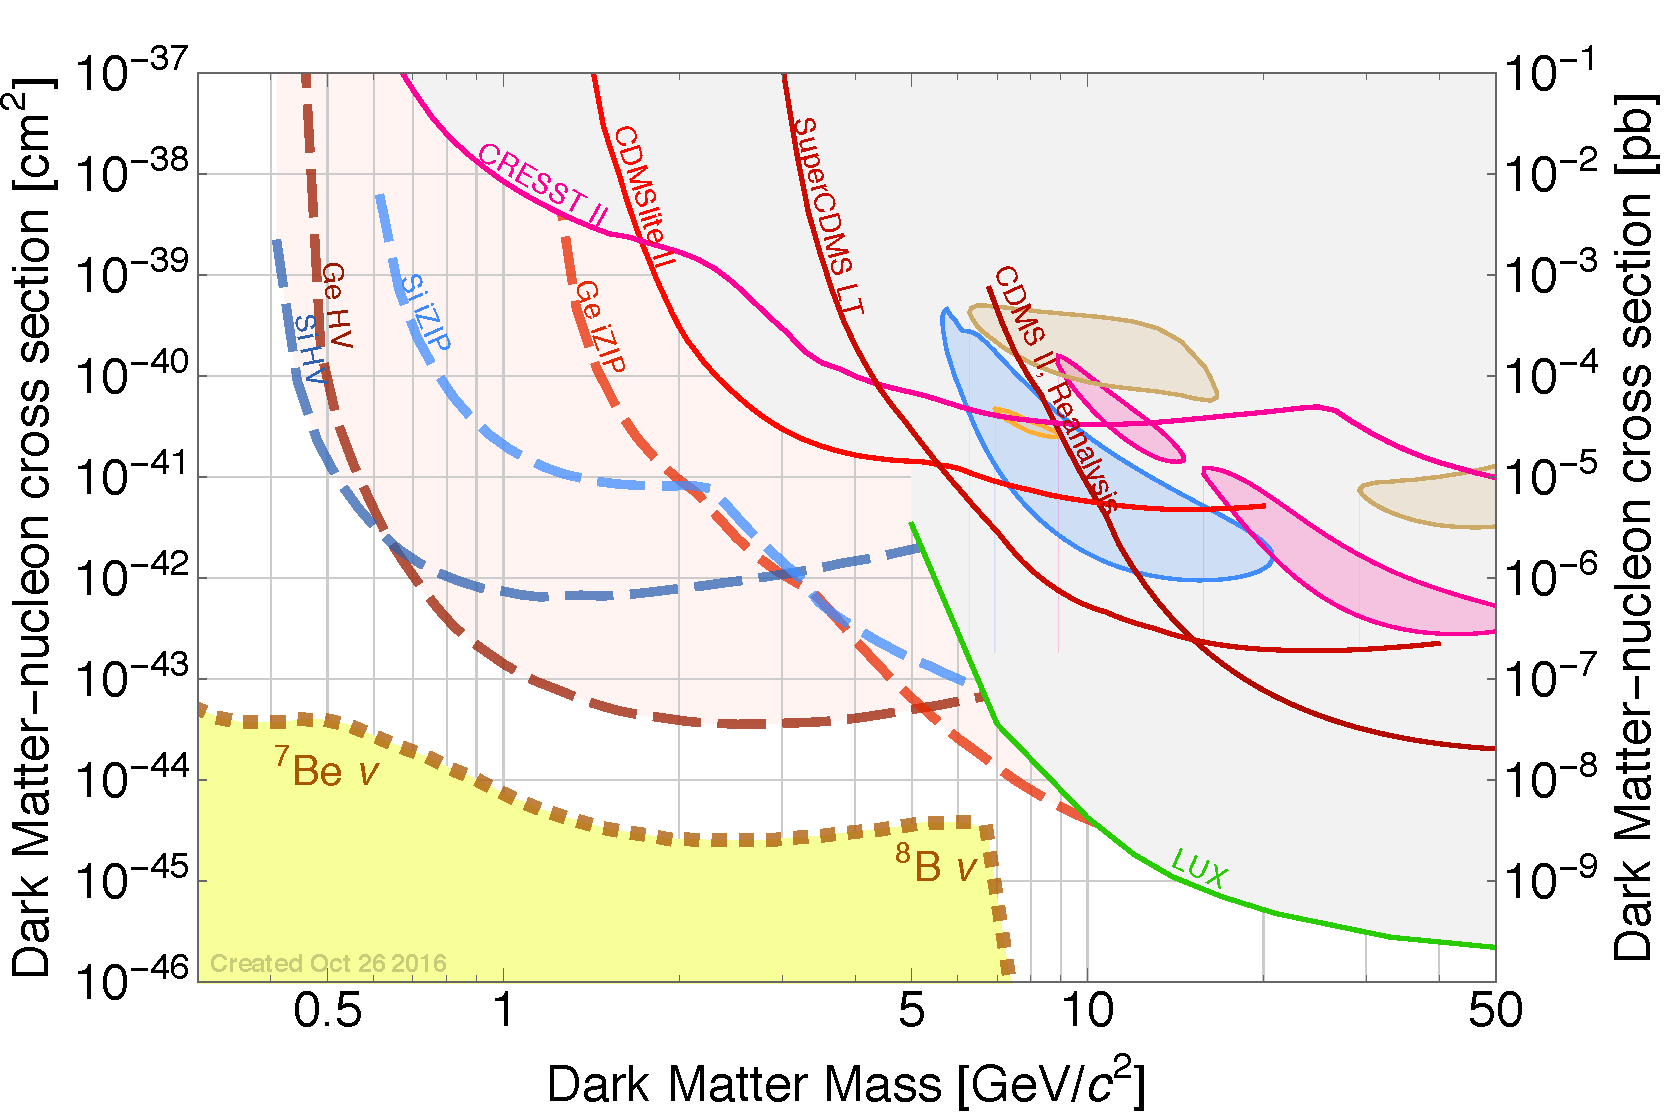
\includegraphics[width=\hsize]{Figures/SuperCDMS_Projected_Limits_squat.pdf}
\caption{\footnotesize Projected exclusion sensitivity for the SuperCDMS SNOLAB direct detection dark matter experiment~\cite{SuperCDMSSensitvitiy:2016arXiv}. The vertical axis is the spin-independent dark matter-nucleon cross section under standard halo assumptions ~\cite{Lewin:1995rx}, and the horizontal axis is the dark matter mass, where dark matter is used to mean any low-mass particle dark matter candidate. The blue dashed curves represent the expected sensitivities for the Si HV and iZIP detectors and the red dashed curves the expected sensitivities of the Ge HV and iZIP detectors. These sensitivity limits are determined using the Optimum Interval method~\cite{Yellin:2002xd}, which does not incorporate any knowledge of the specific disposition and source of background events observed during the experimental operation. The solid lines are the current experimental exclusion limits in the low-mass region, from the CRESST-II ~\cite{2012EPJC...72.1971A}, SuperCDMS \cite{Agnese:2014aze,Agnese:2015nto} and LUX ~\cite{Akerib:2015rjg} experiments. The dotted orange line is the DM discovery limit from~\cite{Ruppin:2014bra}, which represents the cross-section at which the interaction rate from dark matter particles becomes comparable to the solar neutrino coherent elastic scattering rate.
}
\label{fig:SIdataProjections}
\end{figure}


Over the past two years, the SuperCDMS collaboration has lead the field in the search for low-mass matter ($<$ 10 GeV/c$^{2}$).  The most recent results from CDMSlite, a mode where the cryogenic germanium detectors are operated at a relatively high bias voltage to amplify the phonon signal reached an energy threshold for electron recoils as low as 56~eV.  Based on 70 kg-days of exposure, these results excluded new parameter space for the dark matter-nucleon spin-independent cross section for dark matter masses between 1.6 and 5.5 GeV/c$^{2}$.  In 2014 the collaboration released results from the first SuperCDMS analysis focused on searching for low mass dark matter using the iZIP detectors.  At the time of publication, this result lead the field.  These results are highlighted in Figure~\ref{fig:SIdataProjections}.

Several collaborations (using different target materials and techniques) have reported potential signals of low-mass dark matter. In particular, an annual modulation in the detection rate was observed by the DAMA/LIBRA collaboration using NaI(Tl)~\cite{Bernabei:03rnc,Bernabei:08epjc}. %as target and has been later confirmed by the extended experiment DAMA/LIBRA~\cite{Bernabei:03rnc,Bernabei:08epjc} reaching a statistical significance of 9.3\,$\sigma$. 
Also, CoGeNT~\cite{Aalseth:11prl2,Aalseth:11prl,Aalseth:13prd}  (using a germanium target) and CDMS II ~\cite{Agnese:13prl} (with data from the Si detectors) have excesses in their data that are compatible with light dark matter with a mass of the order of 10~GeV/c$^2$. 
These observations are challenged by the negative results obtained by other experimental collaborations. 
XENON10, XENON100, LUX ~\cite{Angle:11prl,Aprile:12prl,Akerib:14prl} (based on Xe), the above mentioned germanium-based
CDMS II, EDELWEISS~\cite{Ahmed:2011gh}, and SuperCDMS Soudan~\cite{Agnese:13prl2,Agnese:2014aze}, as well as KIMS (with CsI), CRESST~\cite{Angloher:2014myn} (with CaWO$_4$),
PICASSO~\cite{Archambault:2012pm} (with C$_4$F$_{10}$), PICO 2L~\cite{Amole:2015lsj} (with C$_3$F$_{8}$), SIMPLE~\cite{Felizardo:2011uw}
(with C$_2$ClF$_5$) and COUPP~\cite{Behnke:2012ys} (with CF$_3$I) have obtained 
negative results, setting more stringent upper bounds on the 
dark matter-nucleon cross section. Figure~\ref{fig:SIdataProjections} illustrates the experimental landscape for the dark matter-nucleus spin-independent scattering cross section as a function of the dark matter mass.

%\section{SuperCDMS SNOLAB}
%The SuperCDMS SNOLAB experiment will be a next-generation (G2) direct dark matter search to explore the light mass (1-10~GeV/c$^2$) DM region, and ultimately reach the solar neutrino floor. The SuperCDMS SNOLAB project is being designed to provide a large, shielded, ultra-low-background cryostat capable of housing up to 186 solid state cryogenic detectors (31 towers) operating at temperatures in the 15-40 mK range. The initial SuperCDMS SNOLAB project baseline will have a 29\,kg payload, consisting of 2 towers of 4 Ge (11.1\,kg) and 2 Si (2.4\,kg) detectors operated in the ultra low energy threshold high-voltage CDMSlite mode (CDMS-HV), providing the best sensitivity for DM masses below $\sim$5~GeV/c$^2$, and an additional 2 towers of germanium and silicon iZIP detectors, which provide better sensitivity in the 5-10~GeV/c$^2$ mass range. Assuming 5 years of operation with 80\% livetime, we would obtain raw exposures of 44 kg-yr (Ge HV), 10 kg-yr (Si HV), 56 kg-yr (Ge iZIP), and 5 kg-yr (Si iZIP), respectively. The projected sensitivities of the different operation modes for this initial payload are shown by means of red and blue dashed lines in Figure~\ref{fig:SIdataProjections}.

%With these ultra-low backgrounds and ultra-low threshold detectors, this G2 experiment will have unparalleled sensitivity for low-mass dark matter, with two complementary targets (germanium and silicon). The goals is to achieve sensitivities $\sim$100 times better than the current limits at 10\,\gev, increasing to $\sim 10^{5}$ times better sensitivity at $\sim$1\,\gev. 

%The large cryostat and passive shielding provide the capability to expand the detector mass to the necessary level that would allow full exploration of the low-mass DM parameter space down to DM-nucleon cross sections where solar neutrino-nucleus scattering becomes significant (sometimes called the "neutrino floor"). This could be accomplished with a combination of SuperCDMS detector upgrades.

%\begin{figure}[ht]
%\begin{center}
%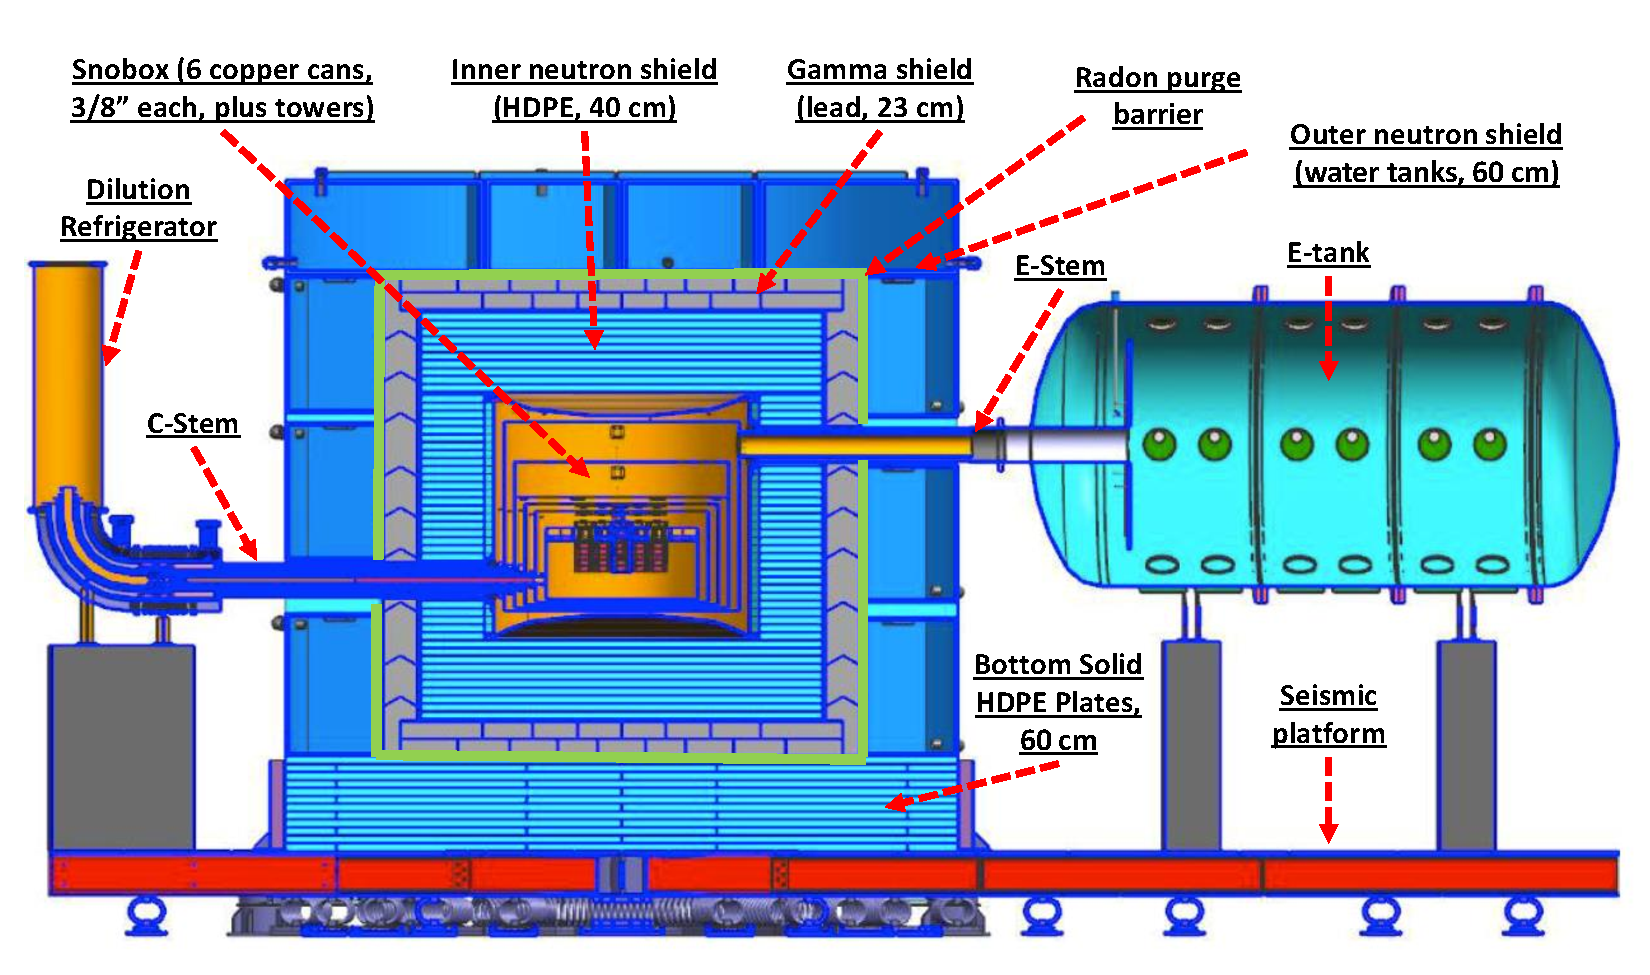
\includegraphics[width=0.8\textwidth]{Figures/f02_SuperCDMS_Schematic.pdf}
%\end{center}
%\caption{\footnotesize Sectional overview of the SuperCDMS SNOLAB conceptual design, showing some of the main features of the cryogenics and shielding systems.}
%\label{fig:overview}
%\end{figure}

%\subsection{\scs Science Goals}
%\label{subsec:science_goals}
%
%In Table~\ref{tab:sciencegoals}, we summarize the science goals for the experiment. We divide our science goals into three categories: primary, secondary, and future capability. The primary science goals drive the technical requirements, while the secondary science goals are examples of the rich set of science the data from this project will provide. The future capability science goal increases the science return from the investment made in the \scs project.
%
%\begin{table}[htbp]
%\centering
%\begin{tabular}{c}
%\hline
%Primary Science Goals \\\hline \\
%\parbox{\textwidth}{\textbf{SG-1} Search for dark matter with mass above 0.5 GeV in a Ge target without background discrimination (see Ge HV curve in Fig.~\ref{fig:SIdataProjections})\vspace{6pt}}\\
%\parbox{\textwidth}{\textbf{SG-2} Search for dark matter with mass above 0.3 GeV in a Si target without background discrimination (see Si HV curve in Fig.~\ref{fig:SIdataProjections})\vspace{6pt}}\\
%\parbox{\textwidth}{\textbf{SG-3} Search for dark matter with mass above 5~GeV in a Ge target with background discrimination (see Ge iZIP curve in Fig.~\ref{fig:SIdataProjections})\vspace{6pt}}\\
%\parbox{\textwidth}{\textbf{SG-4} Search for dark matter with mass above 1~GeV in a Si target with background discrimination (see Si iZIP curve in Fig.~\ref{fig:SIdataProjections})}\\ \\
%\hline 
%Secondary Science Goals \\\hline \\
%\parbox{\textwidth}{\textbf{SG-5} Search for non-standard dark matter interactions within the Effective Field Theory (EFT) framework \vspace{6pt}}\\
%\parbox{\textwidth}{\textbf{SG-6} Observe coherent neutrino scattering of $^8$B solar neutrinos\vspace{6pt}}\\
%\parbox{\textwidth}{\textbf{SG-7} Search for axions produced in the sun and relic axions\vspace{6pt}}\\
%\parbox{\textwidth}{\textbf{SG-8} Search for lightly ionizing particles (LIPS)\vspace{6pt}} \\
%\parbox{\textwidth}{\textbf{SG-9} Search for annual modulation} \\ \\
%\hline
%Future Capability Science Goal \\\hline \\
%\parbox{\textwidth}{\textbf{SG-10} Incorporate a pathway for future upgrades that would further increase the sensitivity of the experiment down to the neutrino floor in this low mass range, including deployment of advanced SuperCDMS detectors or those from the CRESST, EDELWEISS, and EURECA collaborations\vspace{6pt}} \\
%\hline
%\end{tabular}
%\caption{\label{tab:sciencegoals}Science Goals for SuperCDMS SNOLAB}
%\end{table}